\documentclass[../main.tex]{subfiles}


\begin{document}
\section{Segundo apartado}

\subsection{Añadir segundo canal}

En este apartado, se ha realizado la medida de latencia de interrupción usando dos canales del osciloscopio, tras modificar el código fuente del módulo utilizado en el apartado anterior.

\subsection{Modificaciones del código fuente}

El objetivo que se persigue es el mismo: medir la latencia de interrupción. No obstante, ahora se pretende cambiar ligeramente la forma de hacerlo; en el apartado anterior se asume que los pines P9/12 y P9/15 están conectados, de forma que al permutar el valor del pin P9/12 en una función temporizada, se causa una interrupción en el pin P9/15, en cuyo handler se restaura el valor del pin P9/12, de forma que monitorizando el valor de la señal de la conexión entre los pines se tiene en intervalo de tiempo que está el valor permutado la medida de la latencia de interrupción. Pues bien, con esas mismas conexiones entre pines, ahora la función temporizada permutará y restaurará el valor del pin P9/12, causante de la interrupción en el pin P9/15. Por otra parte, el manejador de interrupción permutará y restaurará otro pin del P9, que será monitorizado por otro canal del osciloscopio, de tal forma que el intervalo temporal entre los flancos de subida de las ondas registradas por los dos canales será la medida de la latencia de interrupción.

El pin elegido para ser permutado por el handler de la ISR es el P9/23. Se ha optado por él porque es el que se propone en el guión de la práctica. 

Con el número del pin, P9/23, se va al manual de referencia de la BeagleBone \cite{manual-placa}. Se busca el apartado relativo al \it{expansion header P9}, que está en las páginas 59 a 63 (apartado 6.13.3). En él hay varias tablas, entre las cuales se empieza mirando la 11 (página 59), en la que se nos indica que el nombre de la señal de la placa asociada al pin P9/23 es GPIO1\_17. Tal y como se explica en el guión de la práctica, esto nos permite saber el número con el que ese pin está representado en la interfaz de GPIOs del kernel de Linux; dado que el nombre de la señal es GPIO1\_17, calculando \(1 \cdot 32 + 17 = 49\), se tiene que el pin P9/23 se representa con el número 49. En la tabla 13 (página 62), se indica que para usarlo como GPIO, hay que ponerlo en modo 7 (al igual que pasaba con los pines P9/12 y P9/15). Por otra parte, en la tabla 12 (página 60), está la información de los modos 0 a 3. El modo 0 indica el nombre del registro de control asociado al pin en el SoC de la placa, y en el caso del P9/23, es \it{gpmc\_a1}. Con ese nombre, se va al manual de referencia del SoC de la BeagleBone \cite{manual-soc}. En el apartado 9.3 se listan los registros de control de entrada/salida y su offset sobre la dirección base con el que están mapeados en memoria. Así, en la tabla 10 (página 1459), se indica que el offset del registro de control del GPIO \it{conf\_gpmc\_a1} es \it{844h}.

Con esa información, en la función \it{setup\_pinmux} se configura ahora también el pin P9/23, accediendo a su registro de control mediante \it{AM33XX\_CONTROL\_BASE + 0x844}, y poniéndolo en modo 7, PULLUP, OUTPUT (que es como está configurado el pin P9/12). Es necesario añadir al struct \it{irq\_latency\_test} un campo en el que se almacene el número del pin P9/23 en el interfaz de GPIOs del kernel, de manera análoga a como se hace con los otros dos pines. Después, en la función \it{test\_irq\_latency\_init\_module} hay que programar la solicitud de uso del nuevo pin al kernel, mediante \it{gpio\_request\_one}, con una invocación análoga a la que se hace con el pin P9/12. Por último, en \it{test\_irq\_latency\_exit\_module} hay que comunicar al kernel que se deja de hacer uso del pin P9/23, invocando la función \it{gpio\_free} con el número 49 (que es con el que ese pin se representa).

Con esas modificaciones queda hecha toda la configuración relativa al nuevo pin. Solo falta modificar la función \it{test\_irq\_latency\_timer\_handler} para que restaure el valor del pin P9/12 después de permutarlo. Para que la anchura de la onda se alargue, se ha añadido un bucle que realiza 5000 iteraciones de instrucciones null. Por último, en la función \it{test\_irq\_latency\_interrupt\_handler}, en vez de manipular el pin P9/12, ahora todas las acciones se realizan sobre el pin P9/23, permutando su valor al iniciar la función y restaurándolo antes de hacer el retorno.

\subsection{Preparación de las conexiones al osciloscopio}

La forma de realizar las conexiones del primer canal del osciloscopio es la misma que en el apartado anterior. 

Al añadir el segundo canal, éste debe quedar como se muestra en la siguiente imagen:

\begin{figure}[h]
\centering
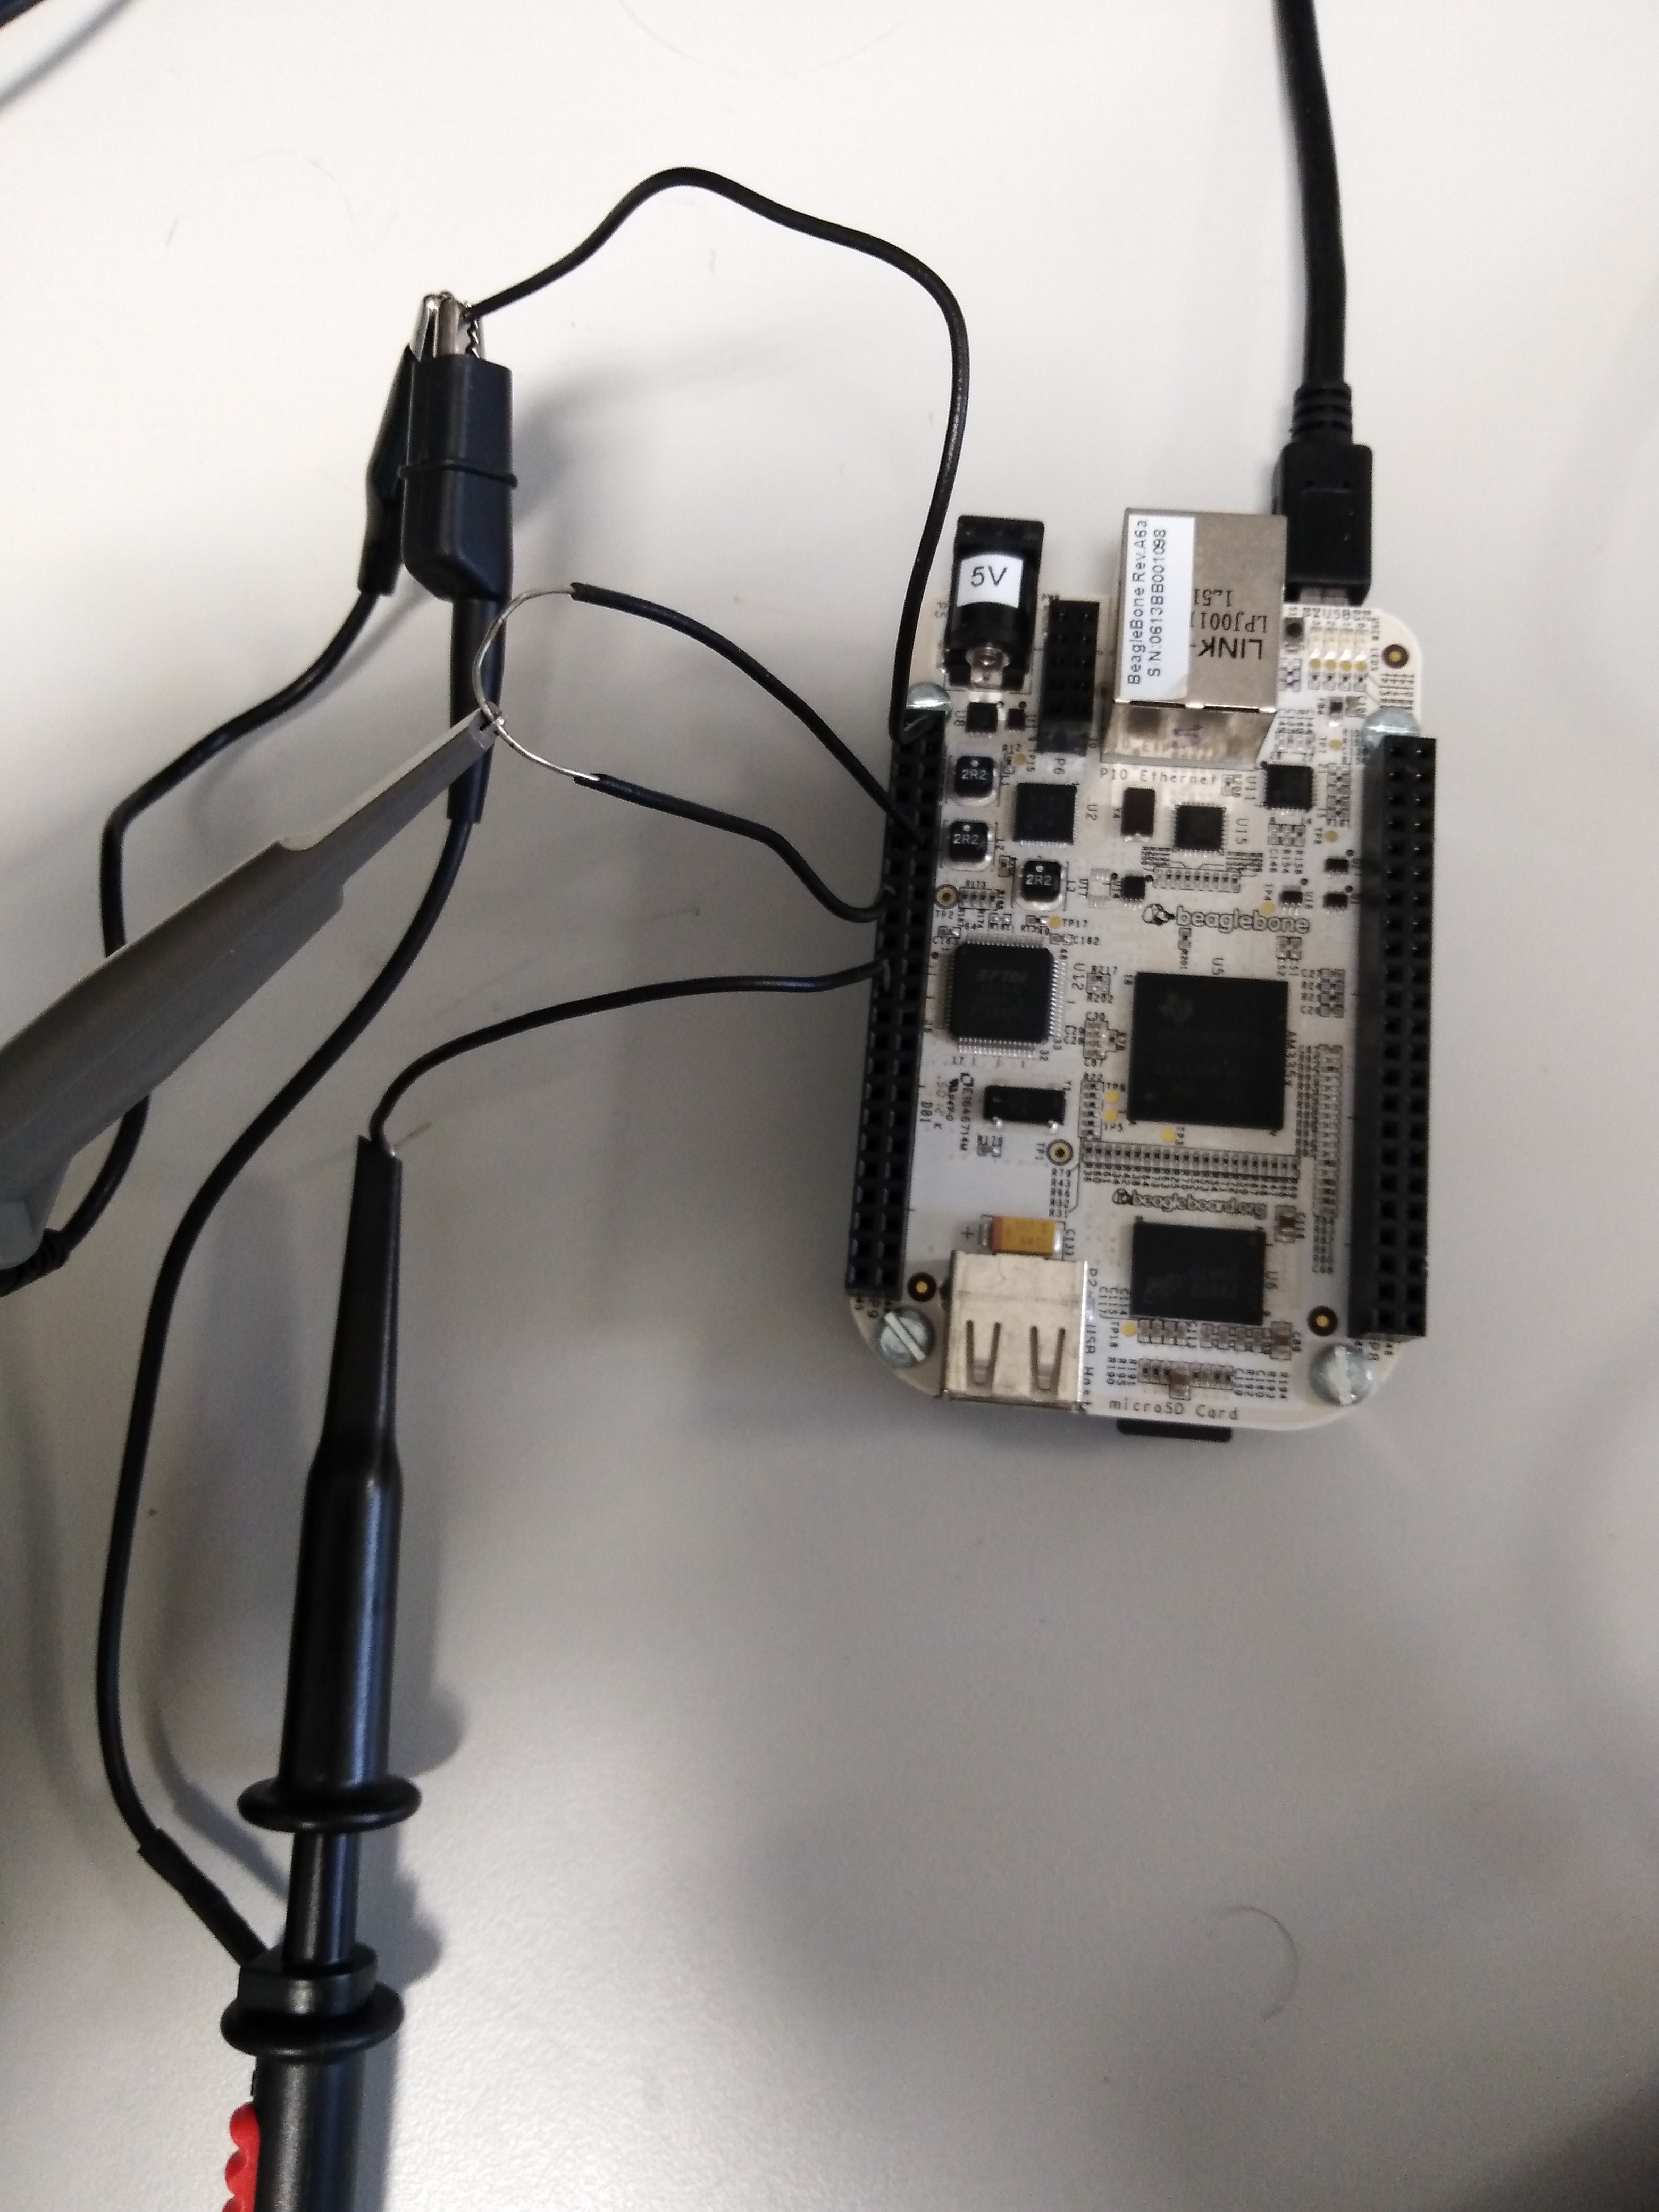
\includegraphics[width=0.5\textwidth]{imagenes/Apartado2-FotografiaPlaca.jpg}
\caption{Fotografía a la placa con las conexiones necesarias al osciloscopio}
\end{figure}

Se puede observar cómo el pin 1, que es la tierra, está conectado a la tierra del segundo canal del osciloscopio, mientras que su sonda está monitorizando el pin 23.

\subsection{Medición de la latencia de interrupción}

Para medir la latencia de interrupción se ha procedido de la misma forma que en el anterior apartado, y se han obtenido los siguientes resultados:

\clearpage % para garantizar que tras lo anterior, va la imagen

\begin{figure}[h]
\centering
\includegraphics[width=1\textwidth]{imagenes/Apartado2-CapturaOsciloscopio.png}
\caption{Fotografía de la pantalla del momento en el que terminan los eventos temporizados}
\end{figure}

Las dos flechas verticales indican el de tiempo que dura la latencia de interrupción, que es el tiempo que pasa desde que la función \it{test\_irq\_latency\_timer\_handler} pone a 1 el valor del pin P9/12, medido por el canal 1 (color azul), y la función \it{test\_irq\_latency\_interrupt\_handler} pone a 1 el valor del pin P9/23, medido por el canal 2 (color rojo).

Nótese cómo, por un descuido de programación, la permutación de valores es de 0 a 1, y no de 1 a 0, como ocurría en el apartado anterior. 

Debido a problemas con el programa picoscope, no se pudo hacer una medición precisa de la latencia sobre la gráfica, pero proporcionalmente, en base la regla en la parte inferior de la ventana, se puede observar como los tiempos de medición de latencia que se tienen son muy parecidos a los que se obtienen por software, al igual que pasaba en el apartado anterior.

\end{document}